\documentclass[twoside]{book}

% Packages required by doxygen
\usepackage{fixltx2e}
\usepackage{calc}
\usepackage{doxygen}
\usepackage[export]{adjustbox} % also loads graphicx
\usepackage{graphicx}
\usepackage[utf8]{inputenc}
\usepackage{makeidx}
\usepackage{multicol}
\usepackage{multirow}
\PassOptionsToPackage{warn}{textcomp}
\usepackage{textcomp}
\usepackage[nointegrals]{wasysym}
\usepackage[table]{xcolor}

% Font selection
\usepackage[T1]{fontenc}
\usepackage[scaled=.90]{helvet}
\usepackage{courier}
\usepackage{amssymb}
\usepackage{sectsty}
\renewcommand{\familydefault}{\sfdefault}
\allsectionsfont{%
  \fontseries{bc}\selectfont%
  \color{darkgray}%
}
\renewcommand{\DoxyLabelFont}{%
  \fontseries{bc}\selectfont%
  \color{darkgray}%
}
\newcommand{\+}{\discretionary{\mbox{\scriptsize$\hookleftarrow$}}{}{}}

% Page & text layout
\usepackage{geometry}
\geometry{%
  a4paper,%
  top=2.5cm,%
  bottom=2.5cm,%
  left=2.5cm,%
  right=2.5cm%
}
\tolerance=750
\hfuzz=15pt
\hbadness=750
\setlength{\emergencystretch}{15pt}
\setlength{\parindent}{0cm}
\setlength{\parskip}{3ex plus 2ex minus 2ex}
\makeatletter
\renewcommand{\paragraph}{%
  \@startsection{paragraph}{4}{0ex}{-1.0ex}{1.0ex}{%
    \normalfont\normalsize\bfseries\SS@parafont%
  }%
}
\renewcommand{\subparagraph}{%
  \@startsection{subparagraph}{5}{0ex}{-1.0ex}{1.0ex}{%
    \normalfont\normalsize\bfseries\SS@subparafont%
  }%
}
\makeatother

% Headers & footers
\usepackage{fancyhdr}
\pagestyle{fancyplain}
\fancyhead[LE]{\fancyplain{}{\bfseries\thepage}}
\fancyhead[CE]{\fancyplain{}{}}
\fancyhead[RE]{\fancyplain{}{\bfseries\leftmark}}
\fancyhead[LO]{\fancyplain{}{\bfseries\rightmark}}
\fancyhead[CO]{\fancyplain{}{}}
\fancyhead[RO]{\fancyplain{}{\bfseries\thepage}}
\fancyfoot[LE]{\fancyplain{}{}}
\fancyfoot[CE]{\fancyplain{}{}}
\fancyfoot[RE]{\fancyplain{}{\bfseries\scriptsize Generated by Doxygen }}
\fancyfoot[LO]{\fancyplain{}{\bfseries\scriptsize Generated by Doxygen }}
\fancyfoot[CO]{\fancyplain{}{}}
\fancyfoot[RO]{\fancyplain{}{}}
\renewcommand{\footrulewidth}{0.4pt}
\renewcommand{\chaptermark}[1]{%
  \markboth{#1}{}%
}
\renewcommand{\sectionmark}[1]{%
  \markright{\thesection\ #1}%
}

% Indices & bibliography
\usepackage{natbib}
\usepackage[titles]{tocloft}
\setcounter{tocdepth}{3}
\setcounter{secnumdepth}{5}
\makeindex

% Hyperlinks (required, but should be loaded last)
\usepackage{ifpdf}
\ifpdf
  \usepackage[pdftex,pagebackref=true]{hyperref}
\else
  \usepackage[ps2pdf,pagebackref=true]{hyperref}
\fi
\hypersetup{%
  colorlinks=true,%
  linkcolor=blue,%
  citecolor=blue,%
  unicode%
}

% Custom commands
\newcommand{\clearemptydoublepage}{%
  \newpage{\pagestyle{empty}\cleardoublepage}%
}

\usepackage{caption}
\captionsetup{labelsep=space,justification=centering,font={bf},singlelinecheck=off,skip=4pt,position=top}

%===== C O N T E N T S =====

\begin{document}

% Titlepage & ToC
\hypersetup{pageanchor=false,
             bookmarksnumbered=true,
             pdfencoding=unicode
            }
\pagenumbering{roman}
\begin{titlepage}
\vspace*{7cm}
\begin{center}%
{\Large Chatting }\\
\vspace*{1cm}
{\large Generated by Doxygen 1.8.11}\\
\end{center}
\end{titlepage}
\clearemptydoublepage
\tableofcontents
\clearemptydoublepage
\pagenumbering{arabic}
\hypersetup{pageanchor=true}

%--- Begin generated contents ---
\chapter{Hierarchical Index}
\section{Class Hierarchy}
This inheritance list is sorted roughly, but not completely, alphabetically\+:\begin{DoxyCompactList}
\item Action\+Listener\begin{DoxyCompactList}
\item \contentsline{section}{osmain.\+Chatting.\+Client\+G\+UI}{\pageref{classosmain_1_1_chatting_1_1_client_g_u_i}}{}
\item \contentsline{section}{osmain.\+Chatting.\+Server\+G\+UI}{\pageref{classosmain_1_1_chatting_1_1_server_g_u_i}}{}
\end{DoxyCompactList}
\item \contentsline{section}{osmain.\+Chatting.\+Chat}{\pageref{classosmain_1_1_chatting_1_1_chat}}{}
\item \contentsline{section}{osmain.\+Chatting.\+Client}{\pageref{classosmain_1_1_chatting_1_1_client}}{}
\item J\+Frame\begin{DoxyCompactList}
\item \contentsline{section}{osmain.\+Chatting.\+Client\+G\+UI}{\pageref{classosmain_1_1_chatting_1_1_client_g_u_i}}{}
\item \contentsline{section}{osmain.\+Chatting.\+Server\+G\+UI}{\pageref{classosmain_1_1_chatting_1_1_server_g_u_i}}{}
\end{DoxyCompactList}
\item Serializable\begin{DoxyCompactList}
\item \contentsline{section}{osmain.\+Chatting.\+Chat\+Message}{\pageref{classosmain_1_1_chatting_1_1_chat_message}}{}
\end{DoxyCompactList}
\item \contentsline{section}{osmain.\+Chatting.\+Server}{\pageref{classosmain_1_1_chatting_1_1_server}}{}
\item Window\+Listener\begin{DoxyCompactList}
\item \contentsline{section}{osmain.\+Chatting.\+Server\+G\+UI}{\pageref{classosmain_1_1_chatting_1_1_server_g_u_i}}{}
\end{DoxyCompactList}
\end{DoxyCompactList}

\chapter{Class Index}
\section{Class List}
Here are the classes, structs, unions and interfaces with brief descriptions\+:\begin{DoxyCompactList}
\item\contentsline{section}{\hyperlink{classosmain_1_1_segmentation_1_1_segment}{osmain.\+Segmentation.\+Segment} }{\pageref{classosmain_1_1_segmentation_1_1_segment}}{}
\item\contentsline{section}{\hyperlink{classosmain_1_1_segmentation_1_1_segmentation}{osmain.\+Segmentation.\+Segmentation} }{\pageref{classosmain_1_1_segmentation_1_1_segmentation}}{}
\end{DoxyCompactList}

\chapter{Class Documentation}
\hypertarget{classosmain_1_1_chatting_1_1_chat}{}\section{osmain.\+Chatting.\+Chat Class Reference}
\label{classosmain_1_1_chatting_1_1_chat}\index{osmain.\+Chatting.\+Chat@{osmain.\+Chatting.\+Chat}}
\subsection*{Static Public Member Functions}
\begin{DoxyCompactItemize}
\item 
static void {\bfseries Chat\+\_\+\+Driver} ()\hypertarget{classosmain_1_1_chatting_1_1_chat_abdead708b3eb0c95958bf220bc4caf95}{}\label{classosmain_1_1_chatting_1_1_chat_abdead708b3eb0c95958bf220bc4caf95}

\end{DoxyCompactItemize}


\subsection{Detailed Description}
\begin{DoxyAuthor}{Author}
Mahmoud Yahia 
\end{DoxyAuthor}


The documentation for this class was generated from the following file\+:\begin{DoxyCompactItemize}
\item 
C\+:/\+Users/\+Mahmoud/\+Desktop/os\+Main/src/osmain/\+Chatting/Chat.\+java\end{DoxyCompactItemize}

\hypertarget{classosmain_1_1_chatting_1_1_chat_message}{}\section{osmain.\+Chatting.\+Chat\+Message Class Reference}
\label{classosmain_1_1_chatting_1_1_chat_message}\index{osmain.\+Chatting.\+Chat\+Message@{osmain.\+Chatting.\+Chat\+Message}}
Inheritance diagram for osmain.\+Chatting.\+Chat\+Message\+:\begin{figure}[H]
\begin{center}
\leavevmode
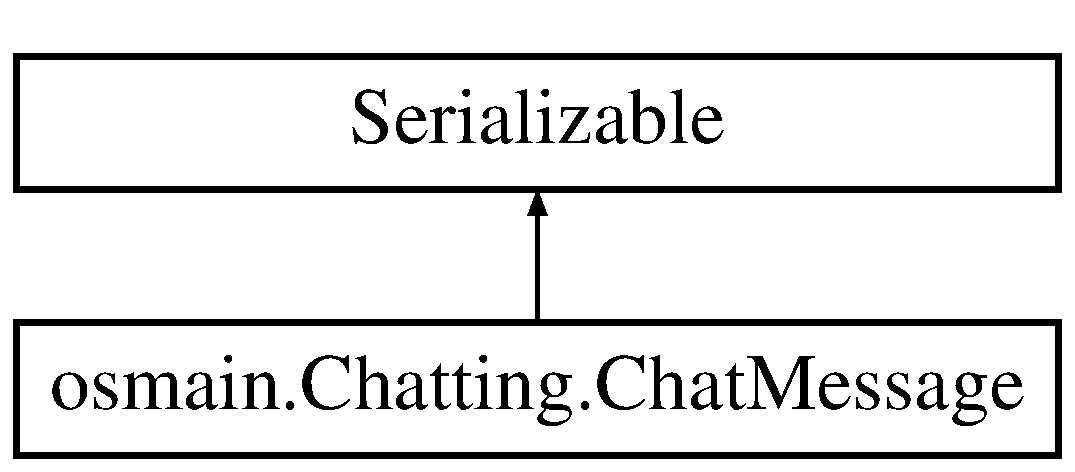
\includegraphics[height=2.000000cm]{classosmain_1_1_chatting_1_1_chat_message}
\end{center}
\end{figure}
\subsection*{Static Protected Attributes}
\begin{DoxyCompactItemize}
\item 
static final long {\bfseries serial\+Version\+U\+ID} = 1112122200L\hypertarget{classosmain_1_1_chatting_1_1_chat_message_a3a1f6f0dea7c2eba4e1ad2a5ed7e818d}{}\label{classosmain_1_1_chatting_1_1_chat_message_a3a1f6f0dea7c2eba4e1ad2a5ed7e818d}

\end{DoxyCompactItemize}


The documentation for this class was generated from the following file\+:\begin{DoxyCompactItemize}
\item 
C\+:/\+Users/\+Mahmoud/\+Desktop/os\+Main/src/osmain/\+Chatting/Chat\+Message.\+java\end{DoxyCompactItemize}

\hypertarget{classosmain_1_1_chatting_1_1_client}{}\section{osmain.\+Chatting.\+Client Class Reference}
\label{classosmain_1_1_chatting_1_1_client}\index{osmain.\+Chatting.\+Client@{osmain.\+Chatting.\+Client}}
\subsection*{Classes}
\begin{DoxyCompactItemize}
\item 
class {\bfseries Listen\+From\+Server}
\end{DoxyCompactItemize}
\subsection*{Public Member Functions}
\begin{DoxyCompactItemize}
\item 
boolean {\bfseries start} ()\hypertarget{classosmain_1_1_chatting_1_1_client_a6b4287c68b6f77f8b5f8be9b2d2dcd35}{}\label{classosmain_1_1_chatting_1_1_client_a6b4287c68b6f77f8b5f8be9b2d2dcd35}

\end{DoxyCompactItemize}
\subsection*{Static Public Member Functions}
\begin{DoxyCompactItemize}
\item 
static void {\bfseries main} (String\mbox{[}$\,$\mbox{]} args)\hypertarget{classosmain_1_1_chatting_1_1_client_ae57c3fd1f60e39b52df5ff0cbfad6559}{}\label{classosmain_1_1_chatting_1_1_client_ae57c3fd1f60e39b52df5ff0cbfad6559}

\end{DoxyCompactItemize}


The documentation for this class was generated from the following file\+:\begin{DoxyCompactItemize}
\item 
C\+:/\+Users/\+Mahmoud/\+Desktop/os\+Main/src/osmain/\+Chatting/Client.\+java\end{DoxyCompactItemize}

\hypertarget{classosmain_1_1_chatting_1_1_client_g_u_i}{}\section{osmain.\+Chatting.\+Client\+G\+UI Class Reference}
\label{classosmain_1_1_chatting_1_1_client_g_u_i}\index{osmain.\+Chatting.\+Client\+G\+UI@{osmain.\+Chatting.\+Client\+G\+UI}}
Inheritance diagram for osmain.\+Chatting.\+Client\+G\+UI\+:\begin{figure}[H]
\begin{center}
\leavevmode
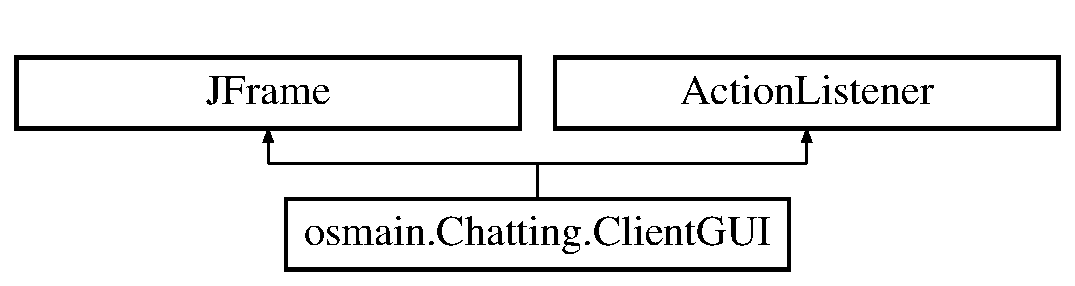
\includegraphics[height=2.000000cm]{classosmain_1_1_chatting_1_1_client_g_u_i}
\end{center}
\end{figure}
\subsection*{Public Member Functions}
\begin{DoxyCompactItemize}
\item 
void {\bfseries action\+Performed} (Action\+Event e)\hypertarget{classosmain_1_1_chatting_1_1_client_g_u_i_aa113754d096807df145c5c98b8909a7b}{}\label{classosmain_1_1_chatting_1_1_client_g_u_i_aa113754d096807df145c5c98b8909a7b}

\end{DoxyCompactItemize}
\subsection*{Static Public Member Functions}
\begin{DoxyCompactItemize}
\item 
static void {\bfseries Client\+G\+U\+I\+\_\+\+Driver} ()\hypertarget{classosmain_1_1_chatting_1_1_client_g_u_i_a2b8416b246420ef0e044b63ef6a32d40}{}\label{classosmain_1_1_chatting_1_1_client_g_u_i_a2b8416b246420ef0e044b63ef6a32d40}

\end{DoxyCompactItemize}


The documentation for this class was generated from the following file\+:\begin{DoxyCompactItemize}
\item 
C\+:/\+Users/\+Mahmoud/\+Desktop/os\+Main/src/osmain/\+Chatting/Client\+G\+U\+I.\+java\end{DoxyCompactItemize}

\hypertarget{classosmain_1_1_chatting_1_1_server}{}\section{osmain.\+Chatting.\+Server Class Reference}
\label{classosmain_1_1_chatting_1_1_server}\index{osmain.\+Chatting.\+Server@{osmain.\+Chatting.\+Server}}
\subsection*{Classes}
\begin{DoxyCompactItemize}
\item 
class {\bfseries Client\+Thread}
\end{DoxyCompactItemize}
\subsection*{Public Member Functions}
\begin{DoxyCompactItemize}
\item 
{\bfseries Server} (int port)\hypertarget{classosmain_1_1_chatting_1_1_server_a65648d064a521815f9e5025b8ec204ae}{}\label{classosmain_1_1_chatting_1_1_server_a65648d064a521815f9e5025b8ec204ae}

\item 
{\bfseries Server} (int port, \hyperlink{classosmain_1_1_chatting_1_1_server_g_u_i}{Server\+G\+UI} sg)\hypertarget{classosmain_1_1_chatting_1_1_server_a959371da05a2e3e1d2ced543510ef02a}{}\label{classosmain_1_1_chatting_1_1_server_a959371da05a2e3e1d2ced543510ef02a}

\item 
void {\bfseries start} ()\hypertarget{classosmain_1_1_chatting_1_1_server_ad513f8dc22d5c97816965f953de6d401}{}\label{classosmain_1_1_chatting_1_1_server_ad513f8dc22d5c97816965f953de6d401}

\end{DoxyCompactItemize}
\subsection*{Static Public Member Functions}
\begin{DoxyCompactItemize}
\item 
static void {\bfseries Server\+\_\+\+Driver} ()\hypertarget{classosmain_1_1_chatting_1_1_server_a803ab6c0cd4610341b305dc147bf786d}{}\label{classosmain_1_1_chatting_1_1_server_a803ab6c0cd4610341b305dc147bf786d}

\end{DoxyCompactItemize}
\subsection*{Protected Member Functions}
\begin{DoxyCompactItemize}
\item 
void {\bfseries stop} ()\hypertarget{classosmain_1_1_chatting_1_1_server_ac31df6bca86cfb36606f3ca82abc0d5e}{}\label{classosmain_1_1_chatting_1_1_server_ac31df6bca86cfb36606f3ca82abc0d5e}

\end{DoxyCompactItemize}


The documentation for this class was generated from the following file\+:\begin{DoxyCompactItemize}
\item 
C\+:/\+Users/\+Mahmoud/\+Desktop/os\+Main/src/osmain/\+Chatting/Server.\+java\end{DoxyCompactItemize}

\hypertarget{classosmain_1_1_chatting_1_1_server_g_u_i}{}\section{osmain.\+Chatting.\+Server\+G\+UI Class Reference}
\label{classosmain_1_1_chatting_1_1_server_g_u_i}\index{osmain.\+Chatting.\+Server\+G\+UI@{osmain.\+Chatting.\+Server\+G\+UI}}
Inheritance diagram for osmain.\+Chatting.\+Server\+G\+UI\+:\begin{figure}[H]
\begin{center}
\leavevmode
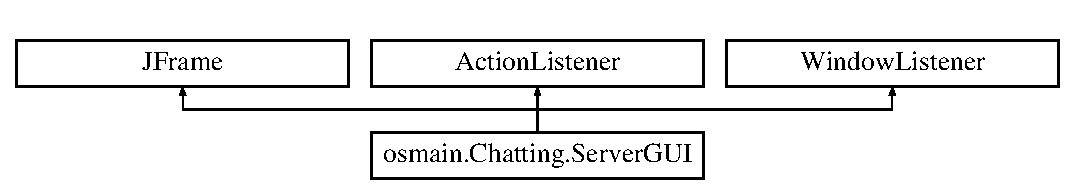
\includegraphics[height=2.000000cm]{classosmain_1_1_chatting_1_1_server_g_u_i}
\end{center}
\end{figure}
\subsection*{Classes}
\begin{DoxyCompactItemize}
\item 
class {\bfseries Server\+Running}
\end{DoxyCompactItemize}
\subsection*{Public Member Functions}
\begin{DoxyCompactItemize}
\item 
void {\bfseries action\+Performed} (Action\+Event e)\hypertarget{classosmain_1_1_chatting_1_1_server_g_u_i_af0aa0016aeb095308931b3d40a9fad15}{}\label{classosmain_1_1_chatting_1_1_server_g_u_i_af0aa0016aeb095308931b3d40a9fad15}

\item 
void {\bfseries window\+Closing} (Window\+Event e)\hypertarget{classosmain_1_1_chatting_1_1_server_g_u_i_a7cc8ba0ac814503cd335bcb7caeb6a72}{}\label{classosmain_1_1_chatting_1_1_server_g_u_i_a7cc8ba0ac814503cd335bcb7caeb6a72}

\item 
void {\bfseries window\+Closed} (Window\+Event e)\hypertarget{classosmain_1_1_chatting_1_1_server_g_u_i_a289c02d7a5788b7c8f7fa5fbee7f29f6}{}\label{classosmain_1_1_chatting_1_1_server_g_u_i_a289c02d7a5788b7c8f7fa5fbee7f29f6}

\item 
void {\bfseries window\+Opened} (Window\+Event e)\hypertarget{classosmain_1_1_chatting_1_1_server_g_u_i_ac21ca7bb05b74cd1c45e1939b32185d3}{}\label{classosmain_1_1_chatting_1_1_server_g_u_i_ac21ca7bb05b74cd1c45e1939b32185d3}

\item 
void {\bfseries window\+Iconified} (Window\+Event e)\hypertarget{classosmain_1_1_chatting_1_1_server_g_u_i_afbc144affd322a79a8095024765872f5}{}\label{classosmain_1_1_chatting_1_1_server_g_u_i_afbc144affd322a79a8095024765872f5}

\item 
void {\bfseries window\+Deiconified} (Window\+Event e)\hypertarget{classosmain_1_1_chatting_1_1_server_g_u_i_a0cb3318dc4bd9113327819a2785221ba}{}\label{classosmain_1_1_chatting_1_1_server_g_u_i_a0cb3318dc4bd9113327819a2785221ba}

\item 
void {\bfseries window\+Activated} (Window\+Event e)\hypertarget{classosmain_1_1_chatting_1_1_server_g_u_i_a9b2ff47e1875a61d7e3dbb47594e5a26}{}\label{classosmain_1_1_chatting_1_1_server_g_u_i_a9b2ff47e1875a61d7e3dbb47594e5a26}

\item 
void {\bfseries window\+Deactivated} (Window\+Event e)\hypertarget{classosmain_1_1_chatting_1_1_server_g_u_i_a2745cc59b31412d3b86afc4792c5e26b}{}\label{classosmain_1_1_chatting_1_1_server_g_u_i_a2745cc59b31412d3b86afc4792c5e26b}

\end{DoxyCompactItemize}
\subsection*{Static Public Member Functions}
\begin{DoxyCompactItemize}
\item 
static void {\bfseries Server\+G\+U\+I\+\_\+\+Driver} ()\hypertarget{classosmain_1_1_chatting_1_1_server_g_u_i_a8e764bc74ca519bba8d77e305ace734d}{}\label{classosmain_1_1_chatting_1_1_server_g_u_i_a8e764bc74ca519bba8d77e305ace734d}

\end{DoxyCompactItemize}


The documentation for this class was generated from the following file\+:\begin{DoxyCompactItemize}
\item 
C\+:/\+Users/\+Mahmoud/\+Desktop/os\+Main/src/osmain/\+Chatting/Server\+G\+U\+I.\+java\end{DoxyCompactItemize}

%--- End generated contents ---

% Index
\backmatter
\newpage
\phantomsection
\clearemptydoublepage
\addcontentsline{toc}{chapter}{Index}
\printindex

\end{document}
